\title{Pevné Látky}
\documentclass[10pt,a4paper]{article}
\usepackage[utf8]{inputenc}
\usepackage[czech]{babel}
\usepackage{amsmath}
\usepackage{amsfonts}
\usepackage{amssymb}
\usepackage{chemfig}
\usepackage{geometry}
\usepackage{wrapfig}
\usepackage{graphicx}
\usepackage{floatflt}
\usepackage{hyperref}
\usepackage{fancyhdr}
\usepackage{tabularx}
\usepackage{makecell}
\usepackage{csquotes}
\usepackage{footnote}
\usepackage{movie15}
\MakeOuterQuote{"}

\renewcommand{\labelitemii}{$\circ$}
\renewcommand{\labelitemiii}{--}
\newcommand{\ra}{$\rightarrow$ }
\newcommand{\x}{$\times$ }
\newcommand{\lp}[2]{#1 -- #2}
\newcommand{\timeline}{\input{timeline}}


\geometry{lmargin = 0.8in, rmargin = 0.8in, tmargin = 0.8in, bmargin = 0.8in}
\date{\today}
\author{Jakub Rádl}

\makeatletter
\let\thetitle\@title
\let\theauthor\@author
\makeatother

\hypersetup{
colorlinks=true,
linkcolor=black,
urlcolor=cyan,
}



\begin{document}
\maketitle
\tableofcontents
\begin{figure}[b]
Toto dílo \textit{\thetitle} podléhá licenci Creative Commons \href{https://creativecommons.org/licenses/by-nc/4.0/}{CC BY-NC 4.0}.\\ (creativecommons.org/licenses/by-nc/4.0/)
\end{figure}
\newpage


\section{Pevné látky}
\begin{enumerate}
\item Jaká je nejpevnější látka? (tvrdost -- diamant, tah -- pavoučí vlákna, dnes uhlíková nanovlákna, \ldots)
\item Jaká jsou využití křemíku? (polovodiče, silikony, \ldots)
\item Proč mají sněhové vločky pravidelný tvar? (díky úhlům v molekule $H_2O$ tvoří 6-úhelník, krystalizuje okolo krystalizačních jader)
\item Co je to koeficient bezpečnosti? (udává, kolikrát více produkt vydrží oproti tomu, na kolik je hodnocen)
\item Co je to nanotechnologie? (technologie $<$ 100nm např. počítačové čipy)
\end{enumerate}

\section{Struktura pevných látek}
\subsection{Atomy a chemické vazby}
\paragraph{Vazby}
\begin{itemize}
\item \textbf{kovalentní} (nevodiče)
\item \textbf{kovová} (umožňuje volný pohyb elektronů -> vodiče)
\item \textbf{iontová} 
\item slabé (vodíková, \ldots)
\end{itemize}

\paragraph{Rozdělení látek}
\begin{itemize}
\item \textbf{monokrystalické} -- pravidelná struktura (diamant, křemík)
\item \textbf{polykrystalické} -- pravidelná struktura v rozdělených oblastech na mikroskopické úrovni (kovy, led)
\item \textbf{amorfní} -- absolutně nepravidelná struktura (sklo, vosk, makromolekulární látky)
\end{itemize}
Mezi amorfními a polykrystalickými látkami je těžko rozlišitelná hranice.
\begin{itemize}
\item \textbf{směsi} (beton)
\end{itemize}


\subsection{Vlastnosti monokrystalů}
\begin{itemize}
\item \textbf{pravidelnost}
\item \textbf{kmitání atomů} kolem rovnovážných poloh
\end{itemize}

\paragraph{Krystalová mřížka}
\begin{itemize}
\item určuje geometrickou souměrnost
\item 7 soustav (matematicky dokázáno, že jich nemůže být více)
\begin{itemize}
	\item krychlová, jednoklonná, trojklonná, klencová, šesterečná, čtverečná, kosočtverečná
\end{itemize}
\end{itemize}

\paragraph{Elementární buňka}
\begin{itemize}
\item základní jednotka krystalu, periodicky se opakuje
\end{itemize}

\paragraph{Př.: železo $\alpha$}\mbox{}\\ \mbox{} \\
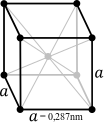
\includegraphics[scale=0.5]{pictures/001.png}
\footnote{https://upload.wikimedia.org/wikipedia/commons/a/a3/Cubic-body-centered.svg}
\begin{itemize}
\item elementární buňkou jsou pouze vnitřní jeden rohový atom
\end{itemize}

\paragraph{Př.: spočítejte hustotu železa z informací o jeho el. buňce}
\begin{itemize}
\item $\rho = \frac{m}{V} = \frac{2 \cdot m_{Fe} }{a^3} = \frac{2 \cdot A_r \cdot m_u }{a^3} = \frac{2 \cdot 56 \cdot 1.66 \cdot 10^{-27}}{(0.287 \cdot 10^{-9})^3} \doteq 7864kg \cdot m^{-3} $
\end{itemize}
pozn.: Struktura a velikost krystalu se určuje pomocí rentgenové difrakce. 

\paragraph{Př.: struktura diamantu}\mbox{}\\ \mbox{} \\
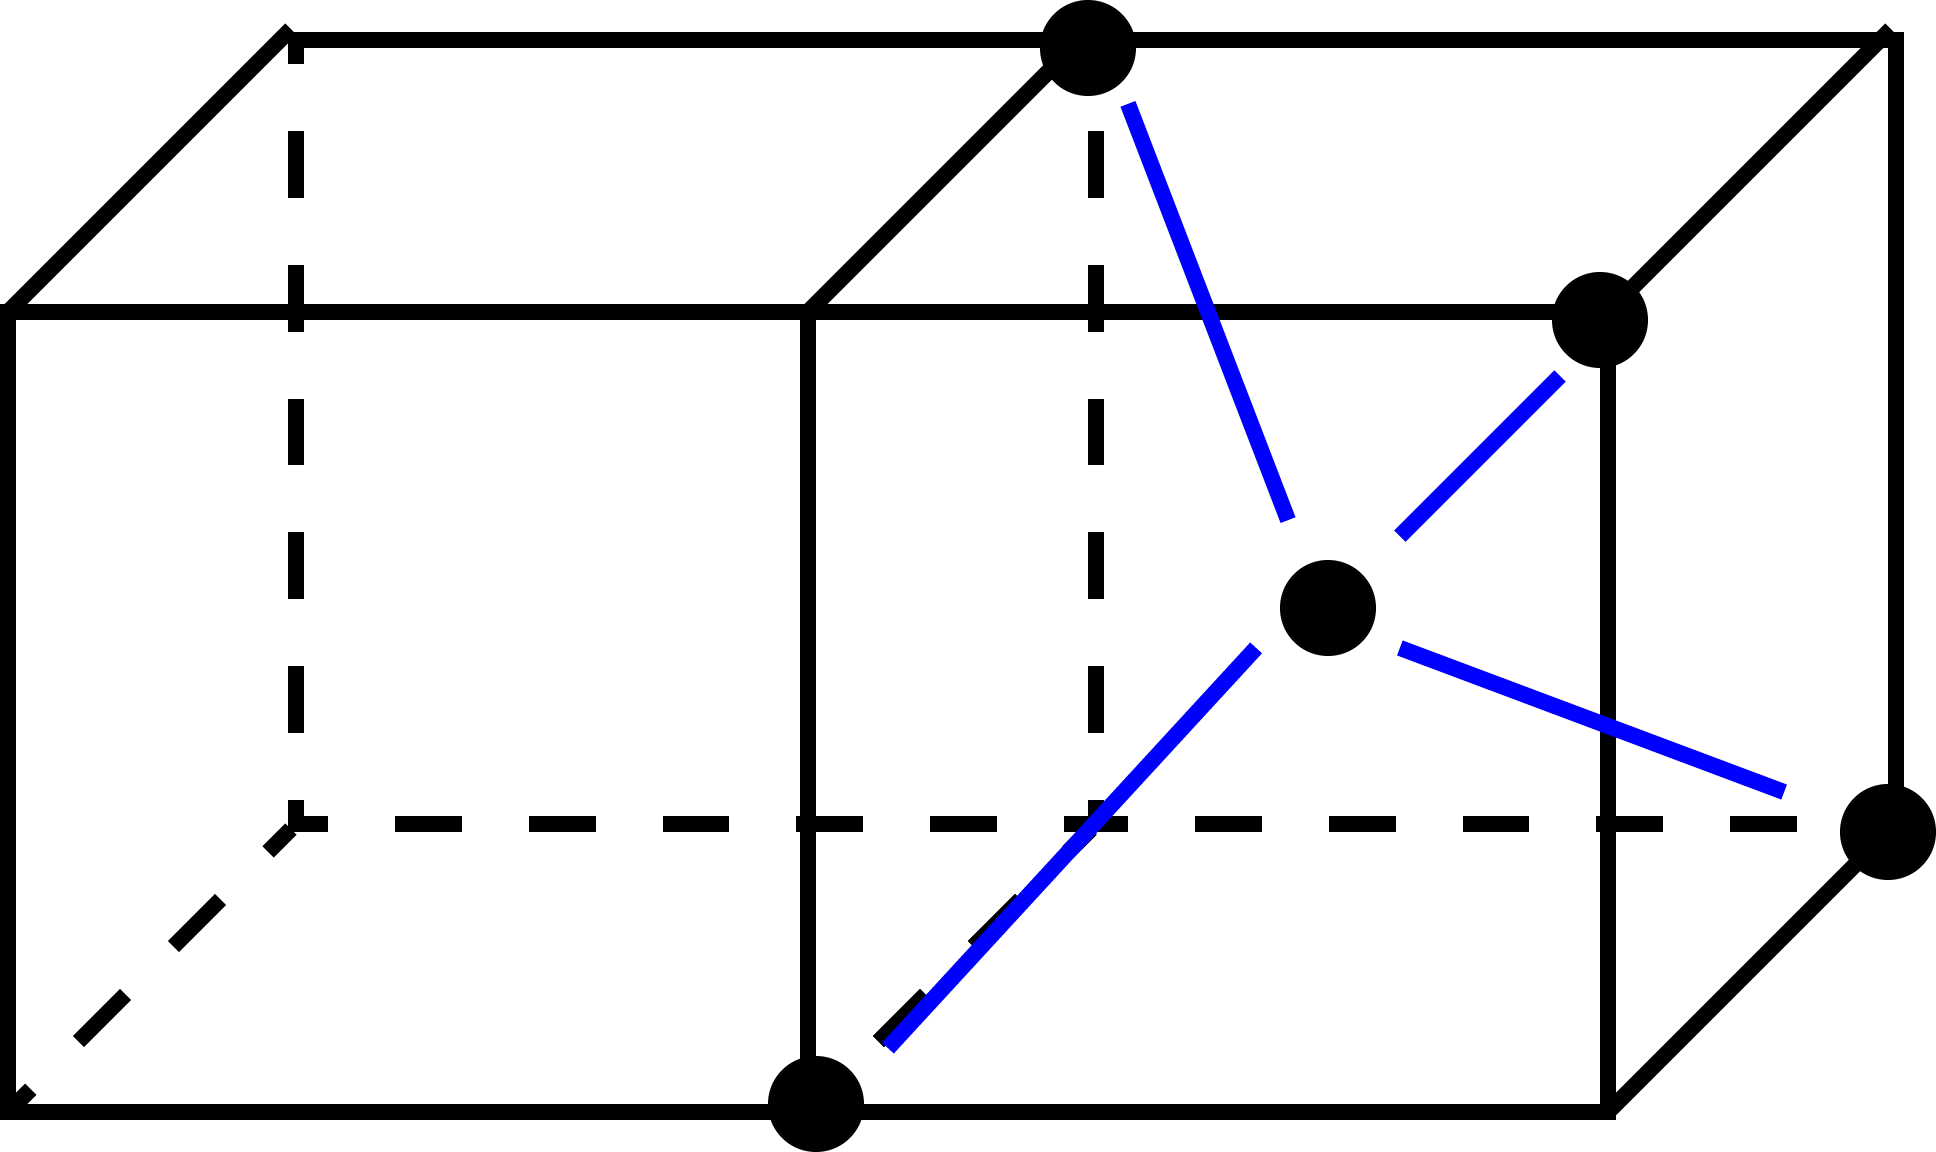
\includegraphics[width=0.25\textwidth]{pictures/002.png}

\paragraph{Př.: struktura fullerenu}\mbox{}\\ \mbox{} \\
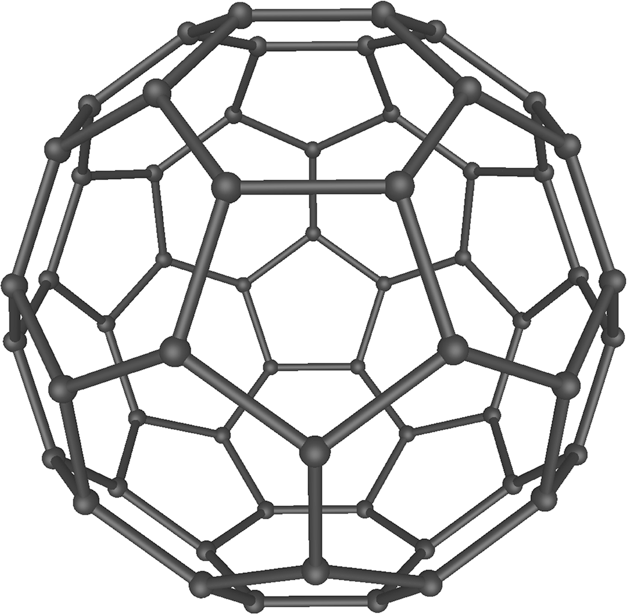
\includegraphics[width=0.25\textwidth]{pictures/003.png}
\footnote{https://upload.wikimedia.org/wikipedia/commons/4/41/C60a.png}

\paragraph{Př.: struktura grafitu}\mbox{}\\ \mbox{} \\
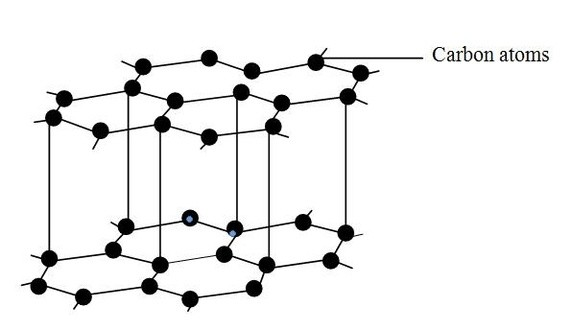
\includegraphics[width=0.4\textwidth]{pictures/004.jpg}
\footnote{https://i.stack.imgur.com/dqwRb.jpg}

\paragraph{Př.: Typy kubické mřížky}
\begin{itemize}
\item[a)] prostá \\
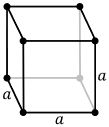
\includegraphics[width=2cm]{pictures/Cubic.png} \footnote{https://upload.wikimedia.org/wikipedia/commons/5/55/Cubic.svg}
\begin{itemize}
\item $a = 2r$ \ldots hrana krychlové mřížky
\item $n = \frac{8}{8} = 1$ \ldots počet atomů (každý z osmi atomů je v osmi buňkách zároveň)
\item $V_{mrizky} = (2r)^3$
\item $V_{atomu} = n \cdot \frac{4}{3} \pi r^3$
\item $\frac{V_a}{V_m} = \frac{\frac{4}{3} \pi r^3}{(2r)^3} = \frac{\pi}{6} \doteq 52\%$
\end{itemize}

\item[b)] plošně centrovaná (v každé stěně jeden navíc) \\
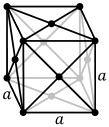
\includegraphics[width=2cm]{pictures/Cubic-face-centered.png} \footnote{https://upload.wikimedia.org/wikipedia/commons/c/c9/Cubic-face-centered.svg}
\begin{itemize}
\item $u = 4r = \sqrt{2}a \Rightarrow a = \sqrt{2}2r$
\item $n = 1+3$ \ldots osm osmin v rozích + půl v každé stěně
\item $\frac{V_m}{V_a} = \frac{4 \cdot (\frac{4}{3}\pi r^3)}{a^3} = \frac{\pi}{3\sqrt{2}} \doteq 0.74\%$
\end{itemize}

\item[c)] prostorově centrovaná (jeden navíc uprostřed) \\
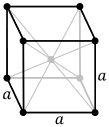
\includegraphics[width=2cm]{pictures/Cubic-body-centered.png} \footnote{https://upload.wikimedia.org/wikipedia/commons/a/a3/Cubic-body-centered.svg}
\begin{itemize}
\item $4r = sqrt(3)a => a = \frac{4}{\sqrt{3}}r$ \ldots prostorová úhlopříčka
\item $n = 2$ \ldots osm osmin v rozích + 1 uprostřed
\item $\frac{V_m}{V_a} = \frac{2 \cdot (\frac{4}{3}\pi r^3)}{a^3} = \frac{\sqrt{3}\pi}{8} \doteq  68\%$
\end{itemize}
\item $\Rightarrow$ plošně centrovaná mřížka je nejefektivnější poskládání atomů (zabírají nejvíce prostoru buňky)
\end{itemize}

\paragraph{Př.: Jak nejefektivněji naskládat atomy}\mbox{} \\ \mbox{} \\
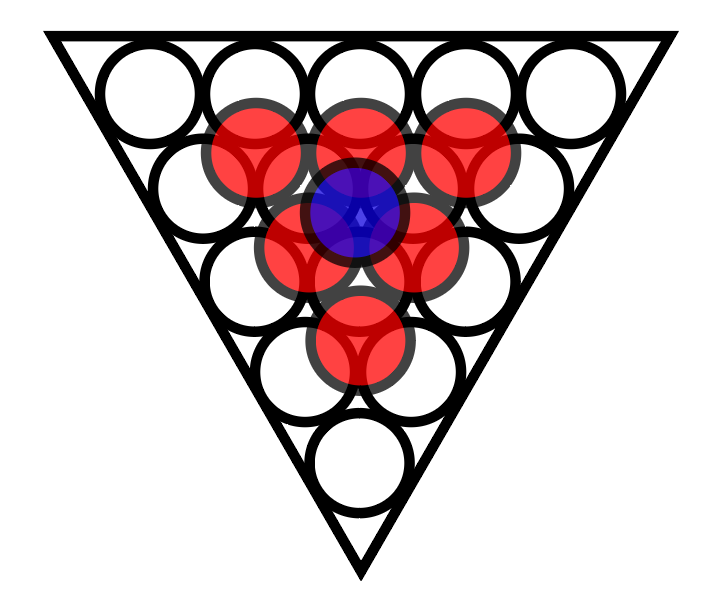
\includegraphics[width=0.3\textwidth]{pictures/004.png}

\subsection{Reálný krystal}
\begin{enumerate}
\item obsahuje příměsi $\rightarrow$ změna vlastností
\item poruchy pravidelnosti
\begin{itemize}
\item dislokace
\end{itemize}
\end{enumerate}



\section{Deformace látek}
\paragraph{Deformace}
\begin{itemize}
\item př.: tahem, tlakem, ohybem, kroucením
\item dělení
	\begin{itemize}
	\item elastická (= vratná)
	\item plastická (= trvalá)
	\end{itemize}
\end{itemize}


\paragraph{Př.: Vlas}
\begin{itemize}
\item $F_{MAX} = 0.8N$ \ldots síla při které se vlas přetrhl
\item $d = 0.07$mm
\item $S = \frac{\pi d^2}{4} = \frac{\pi \cdot (0.07*10^{-3})^2}{4} $
\item $\sigma = \frac{F}{S} = \frac{0.8N}{1.225 \cdot 10^{-9}} = 200MPa$
\end{itemize}

\paragraph{Pevnost látek}
\begin{itemize}
\item závisí na pevnosti chemických vazeb v látce
\end{itemize}


\subsection{Deformace tahem}
\paragraph{Normálové napětí}

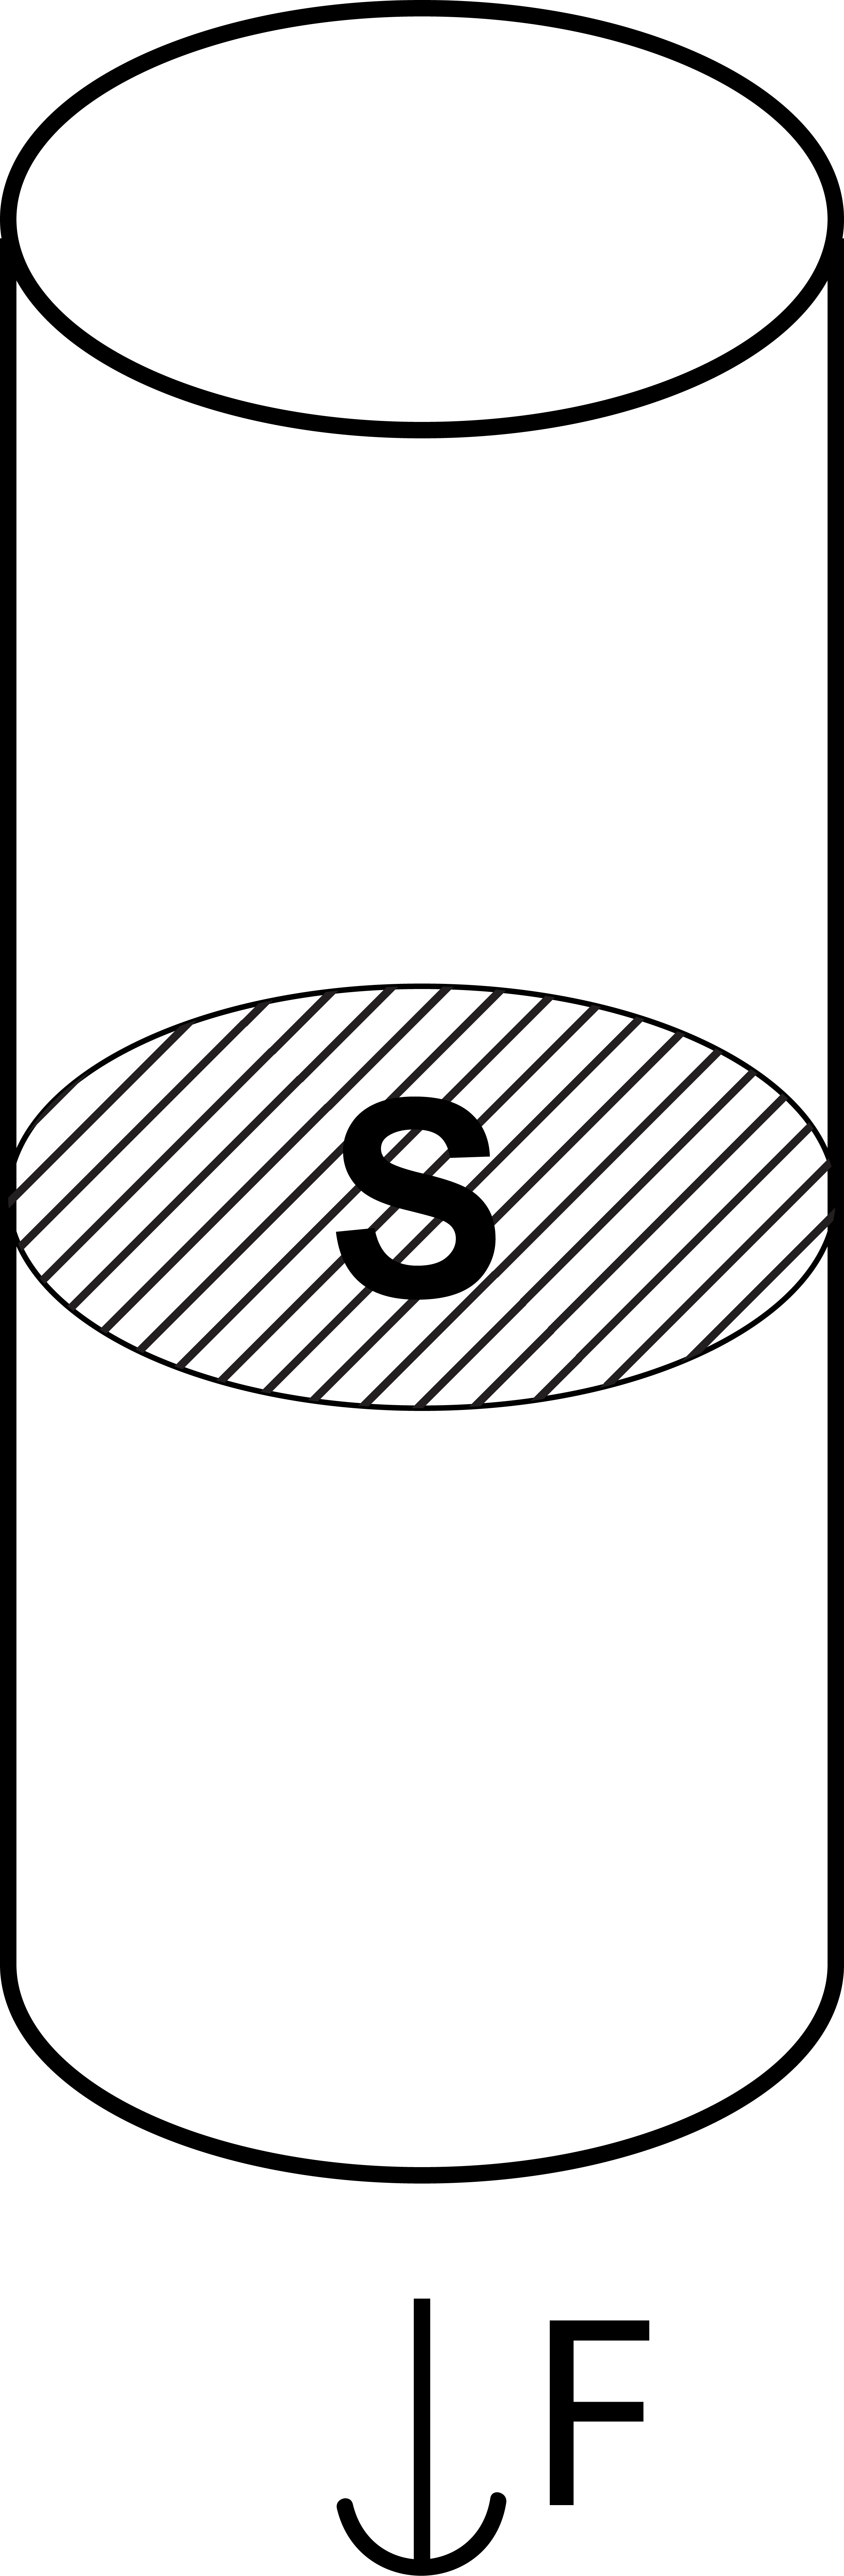
\includegraphics[scale=0.2]{pictures/006.png}

\begin{itemize}
\item $\sigma = \frac{F}{S}$
\item $ [ \sigma ] $ = Pa
\end{itemize}

\paragraph{Hookeův zákon} \mbox{} \\ \mbox{} \\
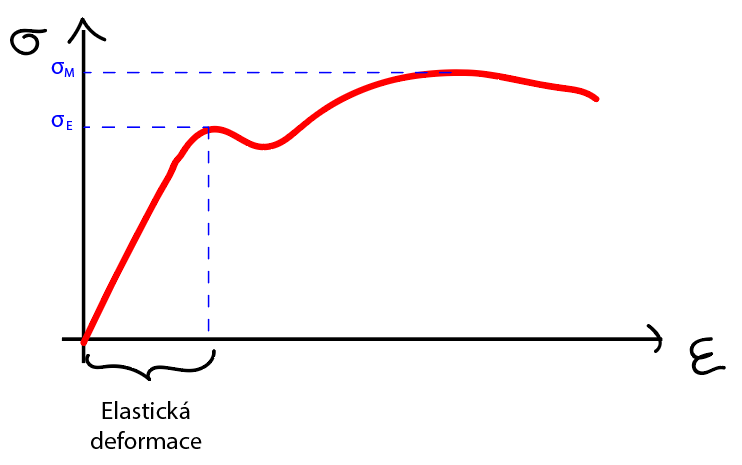
\includegraphics[width=0.5\textwidth]{pictures/005.png}
\begin{itemize}
\item $\varepsilon = \frac{\Delta l}{l}$
\item $\varepsilon$ \ldots relativní prodloužení
\item elastická deformace: $\sigma = E \cdot \varepsilon$
\item $E$ = Youngův model pružnosti
\item $[E]$ = Pa
\end{itemize}

\newpage
\section{Pracovní list -- odpovědi}
\paragraph{Úloha 2}
\begin{enumerate}
\item popisuje geometrickou strukturu
\item kovová, kovalentní, iontová, slabé
\item základní jednotka mřížky
\item kmitají okolo stanovených pozic
\item v krystalické mřížce (diamant -- krychlová, grafit -- šesterečná více vrstev, grafen -- šesterečná jedna vrstva)
\end{enumerate}

\paragraph{Úloha 5}
\begin{enumerate}
\item několikanásobek maximální nosnosti
\item tahem, tlakem, kroucením, \ldots
\item materiál je při ohybu nejnamáhanější nahoře a dole \ra je rozšířený
\item aby byla ohebná a deformace se neprojevovala na celém laně
\item pro lepší pevnost v tahu
\item plastická je vratná, elastická je nevratná a platí Hookův zákon (přímá úměrnost mezi prodloužením a napětím)
\item statické -- pokud zatěžované těleso nezrychluje, dynamické -- pokud ano
\item materiál se namáháním poruší a zničí
\item bude tvrdší a křehčí
\end{enumerate}

\paragraph{Úloha 6}
\begin{itemize}
\item ocel
\item hliník -- kola, pánve, (dural)
\item titan -- pevnost, kluby
\item mosaz -- jemné strojírenství
\item (dřeva, plasty)
\end{itemize}

\paragraph{Úloha 7}
\begin{enumerate}
\item mez pružnosti -- konec lineární části grafu
\item $\sigma = E \cdot \varepsilon \rightarrow E = \frac{\sigma}{\varepsilon} \rightarrow E = \frac{300 \cdot 10^6}{1.5 \cdot 10^{-3}} = 200 * 10^9 $Pa$ = 200$GPa
\item $\varepsilon_{max} = 1.5 \cdot 10^{-3} = 0.15$\%
\item $50 \cdot 0.0015 = 75$mm 
\end{enumerate}

\paragraph{Úloha 14}
\begin{itemize}
\item $\Delta l = \Delta T \cdot \alpha \cdot l_0$ \\ 
$\alpha = \frac{\Delta l}{l_0 \Delta T}$
\end{itemize}



\end{document}